
\documentclass{article}
\usepackage{multirow}
\usepackage{lscape}

%%\input{$HOME/defaults} %$
\title{ Preliminary look at road cost data}

\usepackage{Sweave}
\begin{document}
\maketitle

The World Bank maintains the Road Costs Knowledge (ROCKS) database,
which compiles data on the cost of road construction
projects\footnote{https://www.doingbusiness.org/en/reports/thematic-reports/road-costs-knowledge-system}. ROCKS
was first compiled in 1999, and updated once in 2008 and most recently
in 2018 by the Doing
Business group. The total database covers 3911 road
constructuion  projects in 110 countries. Projects in the
database were started between 1984 and 2017. A single project may
involve multiple components.  A component may be comprised of different
road sections. Work activities in the database are described at the
section level. For example, within the same project, one section of a
road may be widened while the next section may be  graded or
regravelled. Therefore, road work activities at the section level are
the unit of analysis throughout the document. Figure
\ref{fig_world_map} maps the extent of coverage around the
world. Table \ref{tab_count_sources} describes the different types of
data appearing in the database. Figure \ref{fig_cost_distribution}
presents a first look at the distribution of costs. Figure
\ref{fig_estimate_actual} plots actual versus estimated costs for the
557 work activities where the data exists. Finally,
\ref{fig_cost_length_overrun} plots the discrepancies between planned
and estimated costs against discrepancies in planned and estimated
road length.

\begin{figure}
  \caption{Number of work activities per country in ROCKS database}
\label{fig_world_map}
\makebox[\textwidth][c]{
  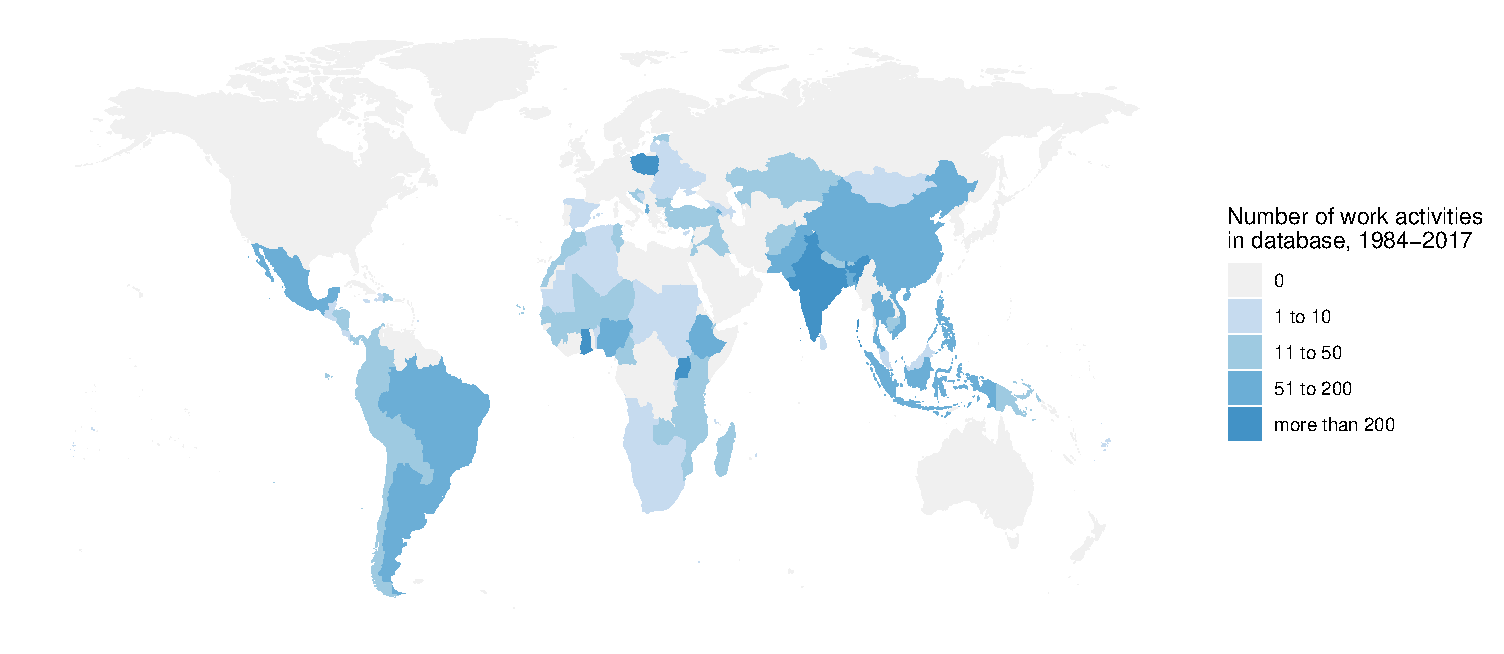
\includegraphics[width = 1.6\textwidth]{figures/coverage_map.pdf}
  }
\end{figure}

% latex table generated in R 3.6.1 by xtable 1.8-4 package
% Wed Sep  4 20:40:41 2019
\begin{table}[ht]
\centering
\caption{Different sources of data. ROCKS compiles data from sources that include project propsals contracts, and evaluations. Projects appearing in the database may have information based on estimates, details of the signed contract, actual costs evaluated after project completion or some combination of the three. \vspace{1em}} 
\label{tab_count_sources}
\begin{tabular}{rrr|lll}
   \hline
\multicolumn{3}{p{6cm}|}{\textbf{Number of activities with data}}  & \multicolumn{3}{p{5cm}}{\textbf{Type of data recorded}}  \\ 
   & cost & length of road & estimated & contract & actual \\ 
   & 1639 & 943 & x &  &  \\ 
   & 1009 & 1006 &  & x &  \\ 
   & 1104 & 892 &  &  & x \\ 
   & 0 & 0 & x & x &  \\ 
   & 557 & 557 & x &  & x \\ 
   & 0 & 0 &  & x & x \\ 
   & 0 & 0 & x & x & x \\ 
   \hline
\textbf{Total} & \textbf{4309} & \textbf{3398} &  &  &  \\ 
   \hline
\end{tabular}
\end{table}



\begin{landscape}
\begin{figure}
  \caption{Distribution of project costs}
\label{fig_cost_distribution}
\makebox[\linewidth][c]{
  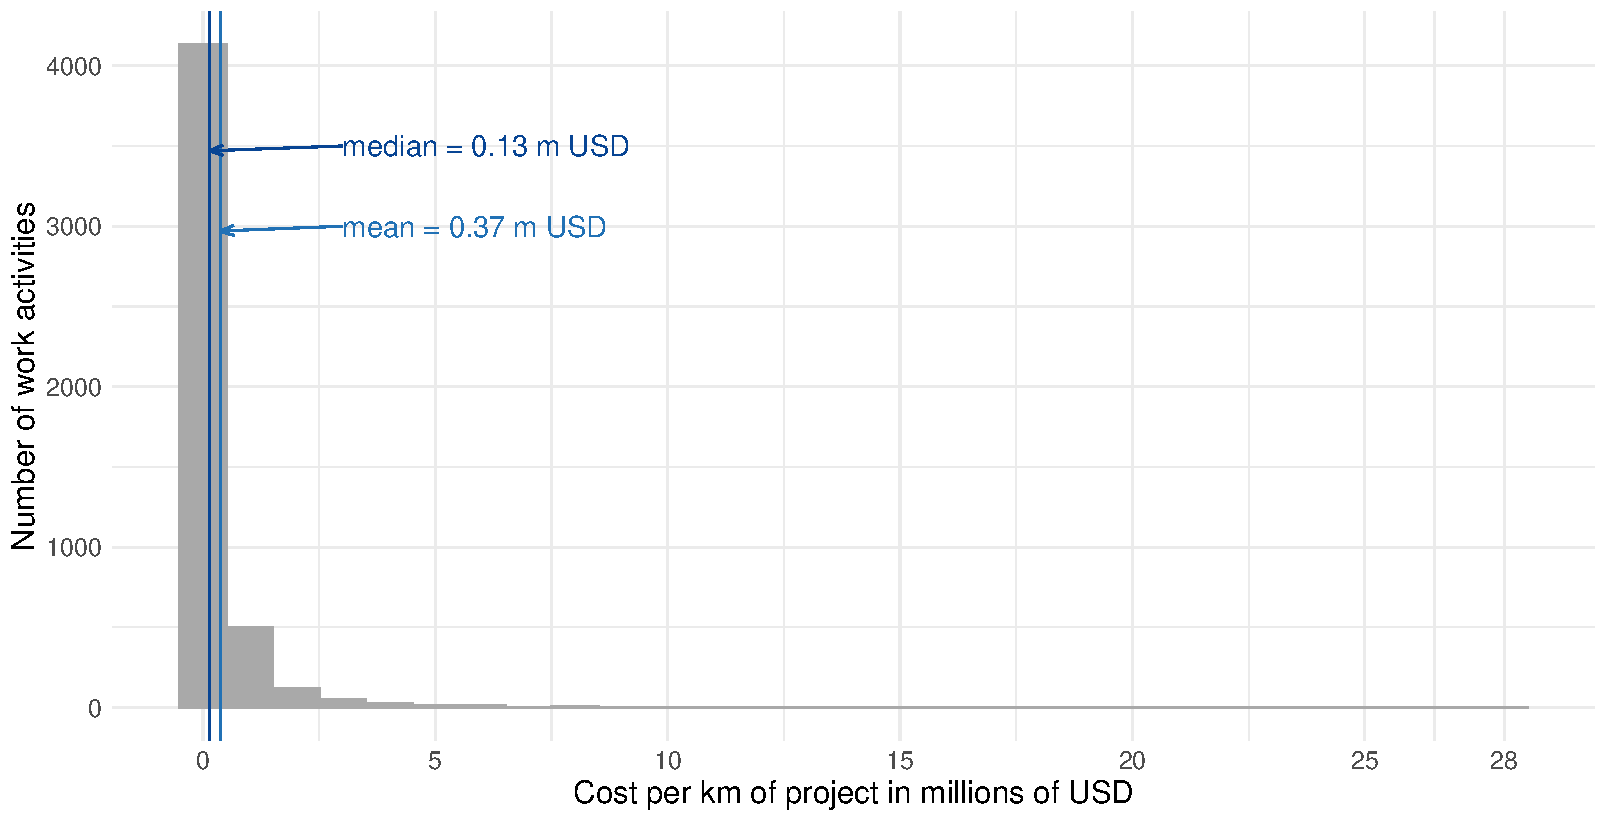
\includegraphics[width = 2\textwidth]{figures/cost_histogram.pdf}
  }
\end{figure}


\begin{figure}
  \caption{Estimated against actual costs}
\label{fig_estimate_actual}
\makebox[\linewidth][c]{
  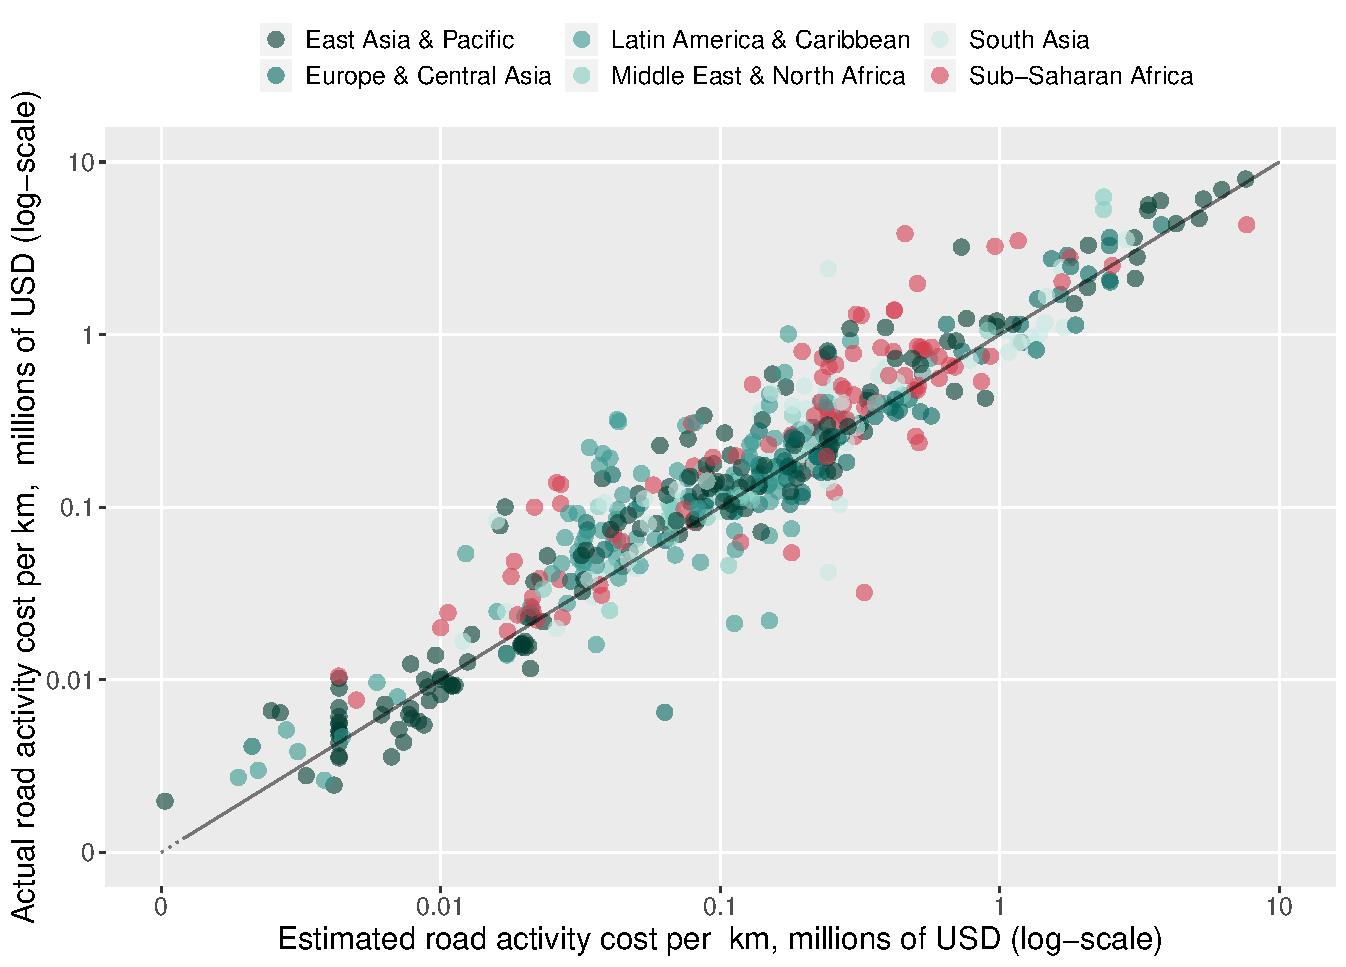
\includegraphics[width = 1.5\textwidth]{figures/estimate_actual.pdf}
  }
\end{figure}

\begin{figure}
  \caption{Cost and length overruns}
\label{fig_cost_length_overrun}
\makebox[\linewidth][c]{
  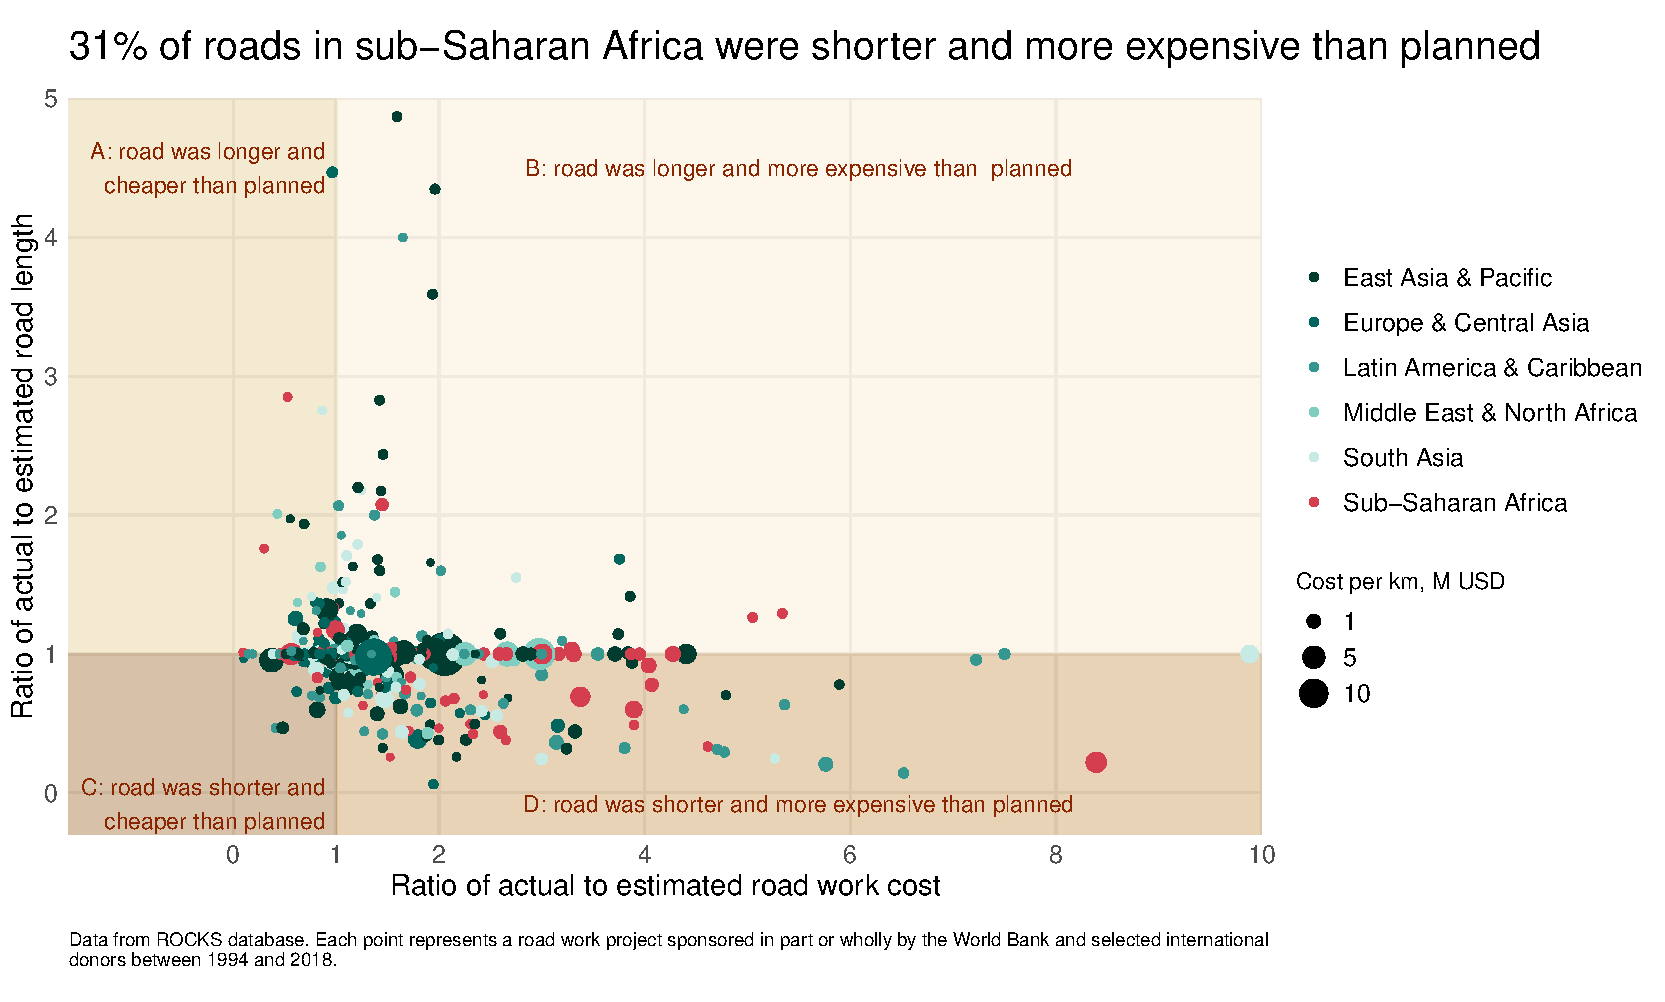
\includegraphics[width = 2\textwidth]{figures/road_cost_length_overrun.pdf}
  }
\end{figure}

\end{landscape}


\end{document}
